
\begin{tabular}{p{7cm}p{4.5cm}p{5cm}}
	Kompensation mit C &
    	\begin{minipage}{4cm}
        	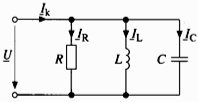
\includegraphics[width=3.5cm]{../WS_DST/bilder/Parallelkompensation.png}
        \end{minipage} & 
		Der Kondensator wird parallel dazu geschalten \\ \\
	Zeigerdiagramme Kompensation &
		\begin{minipage}{4.5cm}
        	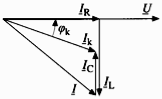
\includegraphics[width=3.5cm]{../WS_DST//bilder/Blindstromkompensation.png}
        \end{minipage} &
		\begin{minipage}{4.5cm}
        	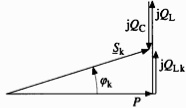
\includegraphics[width=3.5cm]{../WS_DST//bilder/Blindleistungskompensation.png}
        \end{minipage} \\ \\
	Neue (kompensierte) Blindleistung &
		\fbox{$Q_{Lk} = P \cdot \tan{\varphi_k}$} \\ \\
	Blindleistung des Kondensators &
		\fbox{$Q_C = Q_{Lk} - Q_L$} \\ \\
	Kapazit\"at des Kondensators &
		\fbox{$C = -\frac{Q_C}{\omega U^2}$} \\
\end{tabular}